\documentclass[12pt]{article}

% packages
\usepackage[margin=1in]{geometry}
\usepackage[labelfont=it]{caption}
\usepackage{subcaption}
\usepackage{framed}
\usepackage[table]{xcolor}
\usepackage{colortbl, multirow}
\usepackage{amsmath,amsthm,amssymb,wasysym}
\usepackage{mathrsfs, mathtools}
\usepackage{tikz,pgf,pgfplots}
\pgfplotsset{compat=1.16}
\usetikzlibrary{arrows, angles, quotes, decorations.pathreplacing, math, patterns, calc}
\usepackage{graphicx}

% custom commands
\newcommand{\N}{\mathbb{N}}
\newcommand{\Z}{\mathbb{Z}}
\newcommand{\I}{\mathbb{I}}
\newcommand{\R}{\mathbb{R}}
\newcommand{\Q}{\mathbb{Q}}
\newcommand{\p}{^{\prime}}
\newcommand{\powerset}{\raisebox{.15\baselineskip}{\Large\ensuremath{\wp}}}
\DeclarePairedDelimiter{\ceil}{\lceil}{\rceil}
\DeclarePairedDelimiter\floor{\lfloor}{\rfloor}

 
\begin{document}
 
\title{Combinatorial Analysis Example Problems\\
    \large MATH CS 101B Problem Solving II}
\author{Harry Coleman}
\date{January 9, 2020}

\maketitle

\section*{Problem 1}
\fbox{
    \parbox{\textwidth} {
        How many different ordered triples $(a,b,c)$ of nonnegative integers are there such that
        \[a + b + c = 50?\]
    }
}
\\

Since $(a,b,c)$ is an ordered triple, we will consider triples such as
\[(10,20,20) \text{ and } (20,20,10)\]
to be distinct solutions. To represent a particular solution, we will draw out 50 dots, then put two bars somewhere in the line of dots to create three groupings of dots. The first grouping will represent $a$, the second grouping $b$, and the third $c$. The values of each are equal to the number of dots in their respective groupings. An example of this is given in figure \ref{fig:dots-ex}.

\begin{figure}[ht]
    \centering
    
\begin{tikzpicture}
        \foreach \x / \up in {0,...,49}
            \draw[fill=black] (\x/4,0) circle (2pt);
        
        \draw[black] (2.375, 0.5) -- (2.375, -0.5);
        \draw[black] (6.125, 0.5) -- (6.125, -0.5);
    \end{tikzpicture}
    \caption{The dots and bars representing the solution $(10,15,25)$.}
    \label{fig:dots-ex}
\end{figure}

Since $a$, $b$, and $c$ need to be nonnegative, we can allow them to be zero. In a drawing, this would be shown by the left bar having no dots to it's left for $a=0$, no dots between the two bars for $b=0$, and no dots to the right of the right bar for $c=0$. Each of these cases is shown in figure \ref{fig:zero-ex}.

\begin{figure}[ht]
    \centering
    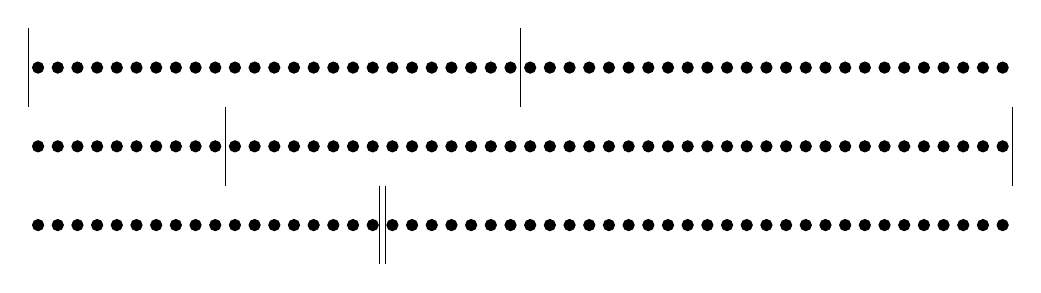
\begin{tikzpicture}
        \foreach \x in {0,...,49}
            \draw[fill=black] (\x/4,0) circle (2pt);
        \foreach \x in {0,...,49}
            \draw[fill=black] (\x/4,1) circle (2pt);
        \foreach \x in {0,...,49}
            \draw[fill=black] (\x/4,2) circle (2pt);
        
        \draw[black] (-0.125, 2.5) -- (-0.125, 1.5);
        \draw[black] (6.125,2.5) -- (6.125, 1.5);
        
        \draw[black] (2.375, 1.5) -- (2.375, 0.5);
        \draw[black] (12.375,1.5) -- (12.375, 0.5);
        
        \draw[black] (4.34, 0.5) -- (4.34, -0.5);
        \draw[black] (4.41, 0.5) -- (4.41, -0.5);
    \end{tikzpicture}
    \caption{The dots and bars for $(0,25,25)$, $(10,40,0)$, and $(18,0,32)$.}
    \label{fig:zero-ex}
\end{figure}

\newpage
We want to know how many ways there are to arrange these dots and bars such that each arrangement gives us a unique solution. Since we have 50 dots, and 2 bars, there would be $52!$ ways to arrange these items. However, this would count each dot at distinct from the all the other dots, and the two bars as distinct from each other. This means that we would be counting a particular arrangement as difference from the same arrangement, but with the locations of the bars swapped.

Since we want to consider each dot and bar as indistinct, we want to divide the total number of arrangements of distinct dots and bars, by the number of ways to arrange the dots, and the number of ways to arrange the bars. This gives us the value
\[\frac{52!}{2!50!}.\]

In general, if we want to find the number of possible ordered $k$-tuples, $(x_1,x_2,\dots,x_k)$ where each $x_i\in\N\cup\{0\}$ and $x_1+x_2+\cdots+x_k = n$ for some $n\in\N$, we use
\[\frac{(n+k-1)!}{(k-1)!n!} = {n+k-1 \choose k-1}.\]

Since we have $n+k-1$ dots and bars to arrange, and we divide out the arrangements of $k-1$ bars and $n$ dots.


\section*{Problem 2}
\fbox{
    \parbox{\textwidth} {
        Define a domino to be a $1 \times 2$ rectangle. In how many ways can an $n \times 2$ rectangle be tiled by dominoes?
    }
}
\\

We will define $D(n)$ to be the function which returns the possible number of domino-tilings for an $n \times 2$ rectangle. We can trivially find $D(n)$ for $n=1$ and $n=1$, shown in figures \ref{fig:dom1} and \ref{fig:dom2}, respectively.

\begin{figure}[ht]
    \centering
    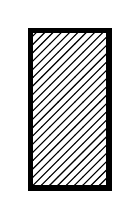
\begin{tikzpicture}
        \draw[line width=2pt, pattern=north east lines] (0,0) rectangle (1,2);
        
    \end{tikzpicture}
    \caption{The possible tiling for $n=1$.}
    \label{fig:dom1}
\end{figure}

\begin{figure}[ht]
    \centering
    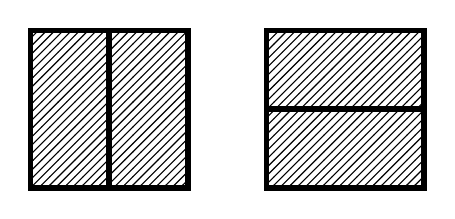
\begin{tikzpicture}
        \draw[line width=2pt, pattern=north east lines] (0,0) rectangle (1,2);
        \draw[line width=2pt, pattern=north east lines] (1,0) rectangle (2,2);
        
        \draw[line width=2pt, pattern=north east lines] (3,0) rectangle (5,1);
        \draw[line width=2pt, pattern=north east lines] (3,1) rectangle (5,2);
        
    \end{tikzpicture}
    \caption{The possible tilings for $n=2$.}
    \label{fig:dom2}
\end{figure}

Now consider a $n\times 2$ rectangle for some arbitrary $n\geq 3$. Each tiling for this rectangle must start with either a vertical domino or two horizontal dominoes, shown in figure \ref{fig:domn}. If we consider the possible tilings of an $n\times 2$ rectangle which start with a vertical domino, we see that there is an $(n-1)\times 2$ rectangle left to tile. The number of ways to tile an $(n-1)\times 2$ is given by $D(n-1)$. So the number of ways to tile an $n\times 2$ rectangle, starting with a vertical domino is $D(n-1)$.

\begin{figure}[ht]
    \centering
    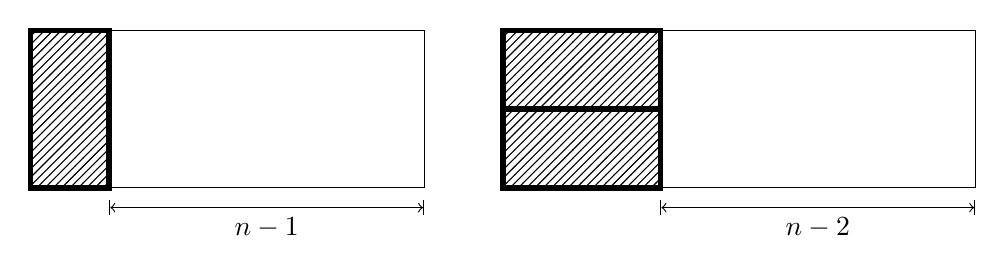
\begin{tikzpicture}
        \draw[line width=2pt, pattern=north east lines] (0,0) rectangle (1,2);
        
        \draw[line width=2pt, pattern=north east lines] (6,0) rectangle (8,1);
        \draw[line width=2pt, pattern=north east lines] (6,1) rectangle (8,2);
        
        \draw[] (1,0) rectangle (5,2);
        \draw[] (8,0) rectangle (12,2);
        
        \draw[|<->|] (1,-0.25) -- (5,-0.25) node[midway, anchor=north]{$n-1$};
        \draw[|<->|] (8,-0.25) -- (12,-0.25) node[midway, anchor=north]{$n-2$};
    \end{tikzpicture}
    \caption{The possible starts for $n\geq 3$.}
    \label{fig:domn}
\end{figure}

Similarly, consider the case that we start with two vertical dominoes. We are left with an $(n-2)\times 2$ rectangle to tile, which has $D(n-2)$ possible tilings. So there are $D(n-2)$ ways to tile an $n\times 2$ rectangle, starting with two horizontal dominoes.

Since a tiling must start with a vertical domino or two horizontal dominoes, then adding these two sets of possible tilings, we find that an $n\times 2$ rectangle can be tiled in a number of ways equal to the sum of the number of possibilities when starting with a vertical tile and the number of possible tilings when starting with two horizontal tiles. This gives us $D(n) = D(n-1) + D(n-2)$. Table \ref{tab:dtab} shows that this rule creates the Fibonacci sequence. 

\begin{table}[ht]
    \centering
    \rowcolors{1}{white}{gray!10}
    \begin{tabular}{c|cccccccccc}
        $n$ & 1 & 2 & 3 & 4 & 5 & 6 & 7 & 8 & 9 & 10 \\
        \hline
        \cellcolor{white} $D(n)$ & 1 & 2 & 3 & 5 & 8 & 13 & 21 & 34 & 55 & 89
    \end{tabular}
    \caption{A few values for $D(n)$}
    \label{tab:dtab}
\end{table}

An explicit formula for this exists, and can also be derived by a different method, similar to that in problem 1. If we consider, again, an $n\times 2$ rectangle. A particular tiling of this rectangle has a number of pairs of horizontal dominoes, call this $x$. $x$ pairs of horizontal dominoes takes up $2x$ units of horizontal space in the rectangle, leaving $n-2x$ units for the vertical dominoes, each with a width of 1. This means there are $n-2x$ vertical dominoes. We now find the number of ways to arrange $x$ indistinct pairs of horizontal dominoes and $n-2x$ indistinct vertical dominoes. This gives us
\[\frac{(n-2x+x)!}{(n-x)!x!} = {n-2x+x \choose x}.\]

Since each pair of horizontal tiles takes up 2 horizontal units, and the rectangle is $n$ units wide, we can tile with up to $\floor{n/2}$ horizontal pairs of dominoes. So to count all possible domino-tilings of an $n\times 2$ rectangle, we use
\[D(n) = \sum_{x=0}^{\floor{n/2}} {n-x \choose x}.\]
Which, indeed, gives us the same values as the recursive formula, $D(n) = D(n-1) + D(n-2)$ with $D(1)=1$ and $D(2) = 2$.


\section*{Problem 5}
\fbox{
    \parbox{\textwidth} {
        Given a unit square, show that if five points are placed anywhere inside or on the border of this square, then two of them must be at most $\sqrt{2}/2$ units apart.
    }
}
\\

Consider the unit square partitioned into 4 squares of half-unit side length, shown in figure \ref{fig:square}.

\begin{figure}[ht]
    \centering
    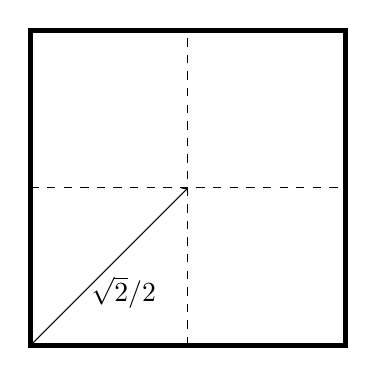
\begin{tikzpicture}
        \draw[line width=2pt] (0,0) rectangle (4,4);
        \draw[dashed] (2,0) -- (2,4);
        \draw[dashed] (0,2) -- (4,2);
        
        \draw[<->] (0,0) -- (2,2) node[midway, anchor=north west, xshift=-10pt]{$\sqrt{2}/2$};
        
    \end{tikzpicture}
    \caption{A unit square.}
    \label{fig:square}
\end{figure}

Since the greatest distance that can exist within one of these sub-squares is its diagonal, then any two points within the same sub-square can be at most $\sqrt{2}/2$ units apart. Since we have 5 points and 4 sub-squares, at least two must be in the same sub-square. This means that two points inside the unit square are at most $\sqrt{2}/2$ units apart.


\newpage
\section*{Problem 6}
\fbox{
    \parbox{\textwidth} {
         Given 25 officers of 5 ranks and from 5 regiments, can they be arranged in a 5-by-5 formation so that in each row and column there is one officer of each rank and one officer from each regiment? (Note: The same problem for 36 officers was posed by Euler in the eighteenth century.)
    }
}
\\

We will indicate each officer's regiment by a letter in $\{A, B, C, D, E\}$ and their rank by a number in $\{1,2,3,4,5\}$. We first consider filling in a $5\times 5$ formation with just the ranks, shown in table \ref{tab:ranks}.

\begin{table}[ht]
    \centering
    \begin{tabular}{ccccc}
        1 & 2 & 3 & 4 & 5 \\
        5 & 1 & 2 & 3 & 4 \\
        4 & 5 & 1 & 2 & 3 \\
        3 & 4 & 5 & 1 & 2 \\
        2 & 3 & 4 & 5 & 1 \\
    \end{tabular}
    \caption{Each row an column contains one officer of each rank.}
    \label{tab:ranks}
\end{table}

It can be seen that each row is the same as the row above it, shifted to the right one place, and the far right looped back to the left. We then create a similar formation of just regiments, which has the same form as the ranks, but flipped horizontally, shown in figure \ref{tab:regim}.

\begin{table}[ht]
    \centering
    \begin{tabular}{ccccc}
        E & D & C & B & A \\
        D & C & B & A & E \\
        C & B & A & E & D \\
        B & A & E & D & C \\
        A & E & D & C & B \\
    \end{tabular}
    \caption{Each row an column contains one officer of each regiment.}
    \label{tab:regim}
\end{table}

For the regiments,  each row is the same as the row above it, shifted to the left one place, and the far left looped back to the right. When we overlay these two tables, we get the 25 officers, all of varying rank and regiment, in formation. This is shown in table \ref{tab:both}.

\begin{table}[ht]
    \centering
    \begin{tabular}{ccccc}
        E1 & D2 & C3 & B4 & A5 \\
        D5 & C1 & B2 & A3 & E4 \\
        C4 & B5 & A1 & E2 & D3 \\
        B3 & A4 & E5 & D1 & C2 \\
        A2 & E3 & D4 & C5 & B1 \\
    \end{tabular}
    \caption{Each row and column contains one officer of each regiment and each rank.}
    \label{tab:both}
\end{table}


\section*{Problem 7}
\fbox{
    \parbox{\textwidth} {
         Consider a block of wood in the shape of a cube, 3 feet on an edge. It is desired to cut the cube into 27 smaller cubes, 1 foot on an edge. What is the smallest number of cuts in which this can be accomplished?
    }
}
\\

If we consider the 3 foot cube as a $3\times 3\times 3$ arrangement of 27 1 foot cubes, we can consider how many cuts it would take to separate any single cube from the rest of the figure. We will consider a cut to be the separation of the figure at a planar intersection. A 1 foot cube at the corner of the 3 foot cube has 3 of its faces already exposed, and would require 3 cuts to create the other 3 faces. A 1 foot cube on the edge of the 3 foot cube has 2 faces already exposed and would require 4 cuts to create the other 4 faces. A 1 foot cube at the center of a face of the 3 foot cube has 1 face exposed and would require 5 cuts. The 1 foot cube at the very center of the 3 foot cube has none of its faces exposed to start and would require 6 cuts to create all of it's faces. Performing these cuts on the cube also properly cuts out the rest of the 1 foot cubes. So 6 cuts is necessary and sufficient.

\end{document}